\begin{frame}{Trellis Diagram}

\begin{center}
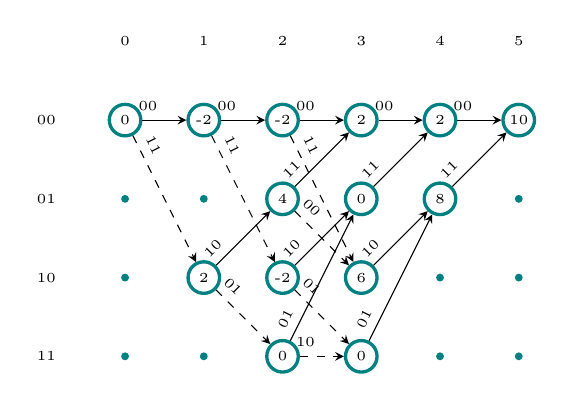
\begin{tikzpicture}[>=stealth, font=\tiny]
\tikzstyle{state} = [draw, circle, teal, very thick, text=black, minimum size=4mm, inner sep=0mm]
\tikzstyle{freestate} = [circle, teal, fill=teal, minimum size=1mm, inner sep=0mm]

 \node[state] (node00) at (0,0) {0} ; \node[freestate] (node10) at (0,-1) {} ; \node[freestate] (node20) at (0,-2) {} ; \node[freestate] (node30) at (0,-3) {} ; \node[state] (node01) at (1,0) {-2} ; \node[freestate] (node11) at (1,-1) {} ; \node[state] (node21) at (1,-2) {2} ; \node[freestate] (node31) at (1,-3) {} ; \node[state] (node02) at (2,0) {-2} ; \node[state] (node12) at (2,-1) {4} ; \node[state] (node22) at (2,-2) {-2} ; \node[state] (node32) at (2,-3) {0} ; \node[state] (node03) at (3,0) {2} ; \node[state] (node13) at (3,-1) {0} ; \node[state] (node23) at (3,-2) {6} ; \node[state] (node33) at (3,-3) {0} ; \node[state] (node04) at (4,0) {2} ; \node[state] (node14) at (4,-1) {8} ; \node[freestate] (node24) at (4,-2) {} ; \node[freestate] (node34) at (4,-3) {} ; \node[state] (node05) at (5,0) {10} ; \node[freestate] (node15) at (5,-1) {} ; \node[freestate] (node25) at (5,-2) {} ; \node[freestate] (node35) at (5,-3) {} ; \node (statelabel0) [left of=node00] {00}; \node (statelabel1) [left of=node10] {01}; \node (statelabel2) [left of=node20] {10}; \node (statelabel3) [left of=node30] {11}; \node (timelabel0) [above of=node00] {0}; \node (timelabel1) [above of=node01] {1}; \node (timelabel2) [above of=node02] {2}; \node (timelabel3) [above of=node03] {3}; \node (timelabel4) [above of=node04] {4}; \node (timelabel5) [above of=node05] {5}; \draw[->] (node00) -- (node01) node [sloped, above, very near start] {00} ; \draw[->, dashed] (node00) -- (node21) node [sloped, above, very near start] {11} ; \draw[->] (node01) -- (node02) node [sloped, above, very near start] {00} ; \draw[->, dashed] (node01) -- (node22) node [sloped, above, very near start] {11} ; \draw[->] (node21) -- (node12) node [sloped, above, very near start] {10} ; \draw[->, dashed] (node21) -- (node32) node [sloped, above, very near start] {01} ; \draw[->] (node02) -- (node03) node [sloped, above, very near start] {00} ; \draw[->, dashed] (node02) -- (node23) node [sloped, above, very near start] {11} ; \draw[->] (node12) -- (node03) node [sloped, above, very near start] {11} ; \draw[->, dashed] (node12) -- (node23) node [sloped, above, very near start] {00} ; \draw[->] (node22) -- (node13) node [sloped, above, very near start] {10} ; \draw[->, dashed] (node22) -- (node33) node [sloped, above, very near start] {01} ; \draw[->] (node32) -- (node13) node [sloped, above, very near start] {01} ; \draw[->, dashed] (node32) -- (node33) node [sloped, above, very near start] {10} ; \draw[->] (node03) -- (node04) node [sloped, above, very near start] {00} ; \draw[->] (node13) -- (node04) node [sloped, above, very near start] {11} ; \draw[->] (node23) -- (node14) node [sloped, above, very near start] {10} ; \draw[->] (node33) -- (node14) node [sloped, above, very near start] {01} ; \draw[->] (node04) -- (node05) node [sloped, above, very near start] {00} ; \draw[->] (node14) -- (node05) node [sloped, above, very near start] {11} ;

\end{tikzpicture}
\end{center}

\end{frame}

\begin{frame}{Trellis Diagram}

\begin{center}
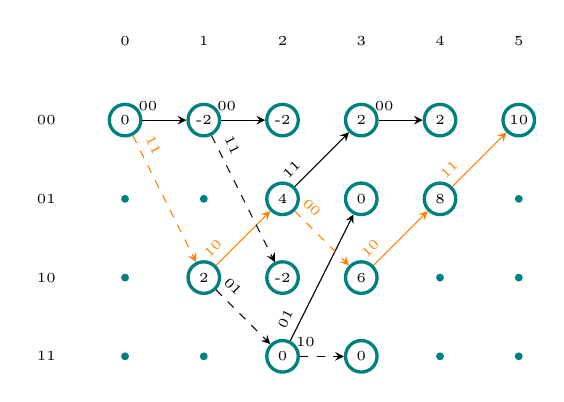
\begin{tikzpicture}[>=stealth, font=\tiny]
\tikzstyle{state} = [draw, circle, teal, very thick, text=black, minimum size=4mm, inner sep=0mm]
\tikzstyle{freestate} = [circle, teal, fill=teal, minimum size=1mm, inner sep=0mm]

 \node[state] (node00) at (0,0) {0} ; \node[freestate] (node10) at (0,-1) {} ; \node[freestate] (node20) at (0,-2) {} ; \node[freestate] (node30) at (0,-3) {} ; \node[state] (node01) at (1,0) {-2} ; \node[freestate] (node11) at (1,-1) {} ; \node[state] (node21) at (1,-2) {2} ; \node[freestate] (node31) at (1,-3) {} ; \node[state] (node02) at (2,0) {-2} ; \node[state] (node12) at (2,-1) {4} ; \node[state] (node22) at (2,-2) {-2} ; \node[state] (node32) at (2,-3) {0} ; \node[state] (node03) at (3,0) {2} ; \node[state] (node13) at (3,-1) {0} ; \node[state] (node23) at (3,-2) {6} ; \node[state] (node33) at (3,-3) {0} ; \node[state] (node04) at (4,0) {2} ; \node[state] (node14) at (4,-1) {8} ; \node[freestate] (node24) at (4,-2) {} ; \node[freestate] (node34) at (4,-3) {} ; \node[state] (node05) at (5,0) {10} ; \node[freestate] (node15) at (5,-1) {} ; \node[freestate] (node25) at (5,-2) {} ; \node[freestate] (node35) at (5,-3) {} ; \node (statelabel0) [left of=node00] {00}; \node (statelabel1) [left of=node10] {01}; \node (statelabel2) [left of=node20] {10}; \node (statelabel3) [left of=node30] {11}; \node (timelabel0) [above of=node00] {0}; \node (timelabel1) [above of=node01] {1}; \node (timelabel2) [above of=node02] {2}; \node (timelabel3) [above of=node03] {3}; \node (timelabel4) [above of=node04] {4}; \node (timelabel5) [above of=node05] {5}; \draw[->] (node00) -- (node01) node [sloped, above, very near start] {00} ; \draw[->, dashed,orange] (node00) -- (node21) node [sloped, above, very near start] {11} ; \draw[->] (node01) -- (node02) node [sloped, above, very near start] {00} ; \draw[->,orange] (node21) -- (node12) node [sloped, above, very near start] {10} ; \draw[->, dashed] (node01) -- (node22) node [sloped, above, very near start] {11} ; \draw[->, dashed] (node21) -- (node32) node [sloped, above, very near start] {01} ; \draw[->] (node12) -- (node03) node [sloped, above, very near start] {11} ; \draw[->] (node32) -- (node13) node [sloped, above, very near start] {01} ; \draw[->, dashed,orange] (node12) -- (node23) node [sloped, above, very near start] {00} ; \draw[->, dashed] (node32) -- (node33) node [sloped, above, very near start] {10} ; \draw[->] (node03) -- (node04) node [sloped, above, very near start] {00} ; \draw[->,orange] (node23) -- (node14) node [sloped, above, very near start] {10} ; \draw[->,orange] (node14) -- (node05) node [sloped, above, very near start] {11} ;

\end{tikzpicture}
\end{center}

\end{frame}

\begin{frame}{State Diagram}

\begin{center}
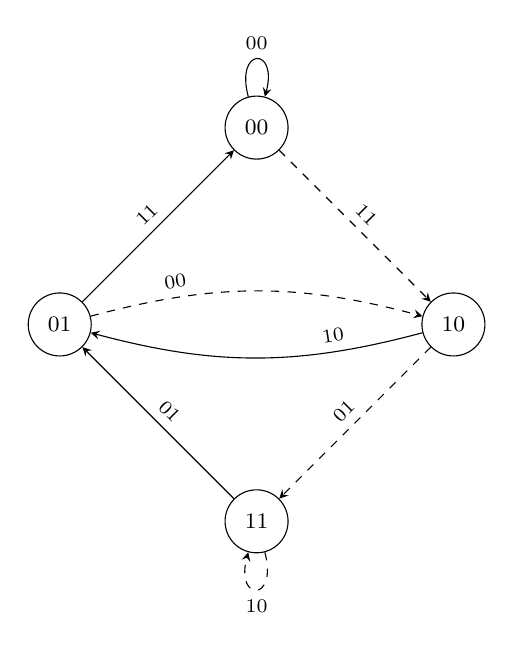
\begin{tikzpicture}[>=stealth, font=\scriptsize]
\tikzstyle{state} = [draw, circle, inner sep=1mm, minimum size=8mm, font=\footnotesize]

 \node[state] (state0) at (0,2.5) {00}; \node[state] (state2) at (2.5,1.53075794227797e-16) {10}; \node[state] (state3) at (3.06151588455594e-16,-2.5) {11}; \node[state] (state1) at (-2.5,-4.59227382683391e-16) {01}; \draw[->] (state0) to [looseness=8,out=105,in=75] node [sloped, above] {00} (state0) ; \draw[->, dashed] (state0) to  node [sloped, above] {11} (state2) ; \draw[->] (state1) to  node [sloped, above] {11} (state0) ; \draw[->, dashed] (state1) to [bend left=15] node [sloped, above,near start] {00} (state2) ; \draw[->] (state2) to [bend left=15] node [sloped, above,near start] {10} (state1) ; \draw[->, dashed] (state2) to  node [sloped, above] {01} (state3) ; \draw[->] (state3) to  node [sloped, above] {01} (state1) ; \draw[->, dashed] (state3) to [looseness=8,out=285,in=255] node [sloped, below] {10} (state3) ;

\end{tikzpicture}
\end{center}

\end{frame}

\begin{frame}{Convolution Encode}

\begin{center}
\begin{minipage}{.4\textwidth}
\begin{center}
\begin{tabular}{c c c c}
  \visible<1-> {state&input&output&next state\\ \hline}
  \visible<2-> {00&1&11&10\\}
  \visible<3-> {10&0&10&01\\}
  \visible<4-> {01&1&00&10\\}
  \visible<5-> {10&0&10&01\\}
  \visible<6-> {01&0&11&00\\}
\end{tabular}
\end{center}
\end{minipage}
\hfill
\begin{minipage}{.4\textwidth}
\begin{center}
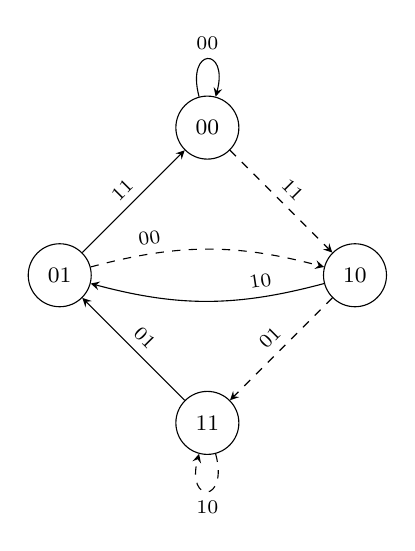
\begin{tikzpicture}[scale=.75, >=stealth, font=\scriptsize]
\tikzstyle{state} = [draw, circle, inner sep=1mm, minimum size=8mm, font=\footnotesize]
 \node[state] (state0) at (0,2.5) {00}; \node[state] (state2) at (2.5,1.53075794227797e-16) {10}; \node[state] (state3) at (3.06151588455594e-16,-2.5) {11}; \node[state] (state1) at (-2.5,-4.59227382683391e-16) {01}; \draw[->] (state0) to [looseness=8,out=105,in=75] node [sloped, above] {00} (state0) ; \draw[->, dashed] (state0) to  node [sloped, above] {11} (state2) ; \draw[->] (state1) to  node [sloped, above] {11} (state0) ; \draw[->, dashed] (state1) to [bend left=15] node [sloped, above,near start] {00} (state2) ; \draw[->] (state2) to [bend left=15] node [sloped, above,near start] {10} (state1) ; \draw[->, dashed] (state2) to  node [sloped, above] {01} (state3) ; \draw[->] (state3) to  node [sloped, above] {01} (state1) ; \draw[->, dashed] (state3) to [looseness=8,out=285,in=255] node [sloped, below] {10} (state3) ;
\end{tikzpicture}
\end{center}
\end{minipage}
\end{center}

\end{frame}
